% The one reproduced plate.
% Rebuilt from its source PDF by tools/relayout_plates.py; see tex/figs/SELECTED.md for the crop
% box and tex/PERMISSIONS.md for the licence it is used under.
%
% A plate is kept only where a photograph or a render carries something a drawing cannot, and
% only where the paper has the right to print it without asking anyone. Everything else that was
% reproduced has been redrawn in the paper's own style (figs/fig_transmission, fig_collision,
% fig_tactiledepth, fig_contactlabel, fig_retarget) or dropped, because the prose already made the
% point or because no honest drawing could be made from what the corpus records. That took
% eighteen plates to one, eleven visual styles to four, and eleven open permissions to none.
%
% The survivor is single column and single panel. It is not a `figure*`: a borrowed plate has not
% earned the page width.
%
% One command for it. A section author places it by writing
%   \plateGraspPenetration
% at the point in the section where the float should be anchored, once: a plate called twice
% prints twice, on two pages, under two numbers.
%
% The plate credits its source inside its own caption with \src or \cite, and carries \licensed as
% well, because its source is CC BY 4.0 and the licence asks for an attribution line.

% ========================================================== Sec. VI, two hands

\newcommand{\plateGraspPenetration}{%
  \begin{figure}[t]
    \centering
    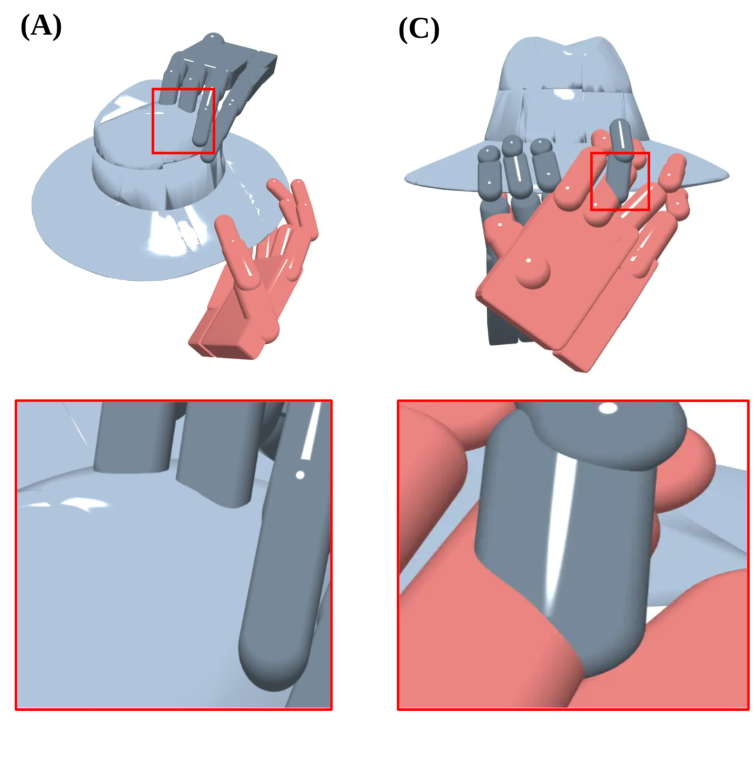
\includegraphics[width=0.86\columnwidth]{figs/selected/bimanual_grasp_penetration.png}
    \caption{Two failures of synthesised two-hand grasps, each enlarged at the
      contact: (A) a finger inside the object, (C) a finger inside the other hand.
      Both look plausible whole~\cite{bimangrasp_2024}.}
    \label{fig:bimanual-penetration}
    \licensed[panels (A) and (C) of Fig.~9]{Fig.~9 of Shao and Xiao, arXiv:2411.15903}{CC BY 4.0}{https://creativecommons.org/licenses/by/4.0/}
  \end{figure}}
